\documentclass[a4paper,oneside,12pt,pdftex]{article}
\usepackage[bahasa]{babel}
\usepackage[top=3cm,left=2.5cm,bottom=3.9cm,right=2.5cm]{geometry}
\usepackage{times}
\usepackage{graphicx}
\usepackage{wrapfig}
\usepackage{subfig}
\usepackage{array}
\usepackage{multirow}
\usepackage{color}
\usepackage{colortbl}
\definecolor{backgroundcolor}{rgb}{0.949019608,0.949019608,0.949019608}
\definecolor{sectioncolor}{rgb}{0.211764706,0.37254902,0.568627451}
\definecolor{subsectioncolor}{rgb}{0.309803922,0.505882353,0.741176471}
\usepackage{hyperref}
\hypersetup{colorlinks,citecolor=blue,filecolor=black,linkcolor=blue,urlcolor=blue,breaklinks=true}
\usepackage{fancyhdr}
\pagestyle{fancy}
\fancyhead{}
\fancyfoot{}
\lfoot
{
\begin{tabular}{|>{\footnotesize}l|}
\hline
\cellcolor{backgroundcolor}Nomor Dokumen: DSG\hspace{2cm}Nomor Revisi: 02\hspace{0.7cm}Tanggal: 17/03/10\hspace{1.5cm}Halaman \thepage\hspace{3pt}dari 12\\
\hline
\end{tabular}\\
{\scriptsize\copyright 2010 oleh LSKK STEI-ITB. Pengungkapan dan penggunaan seluruh isi dokumen hanya dapat dilakukan atas ijin tertulis LSKK STEI-ITB Jalan Ganesha 10 Bandung, 40132 Indonesia.}
}
\renewcommand{\headrulewidth}{0pt}


\begin{document}

\addcontentsline{toc}{section}{Lembar Sampul Dokumen}

\begin{wrapfigure}{l}{0.125\textwidth}
\vspace{-0.5cm}

\includegraphics[height=2.6cm]{Ganesha}
%\rule{\linewidth}{0.2mm}
\end{wrapfigure}
\noindent\textbf{\textsf{\LARGE Dokumen Pengembangan Produk}}\\[0.8cm]
\textsf{\large LAB. SISTEM KENDALI \& KOMPUTER, STEI -- ITB}
\rule{\linewidth}{0.2mm}
\vspace{0.5cm}
\begin{center}
\textbf{\textcolor{sectioncolor}{\textsf{\large Lembar Sampul Dokumen}}}\\[1.1cm]
\end{center}

\arrayrulecolor{white}
\setlength\doublerulesep{11pt}

\begin{tabular}{p{4cm}>{\columncolor{backgroundcolor}}p{10.5cm}}
Judul Dokumen & DOKUMEN DESAIN PRODUK:\\[0.1cm]
 & \cellcolor{backgroundcolor}\emph{PUSPA}\\
\hline\hline
\end{tabular}

\begin{tabular}{p{4cm}p{10.5cm}}
Jenis Dokumen & \cellcolor{backgroundcolor}DSG: DESAIN PRODUK\\
 & \hspace{1.25cm}\textmd{\textsf{\scriptsize Catatan: Dokumen ini dikendalikan penyebarannya oleh LSKK, STEI -- ITB}}\\[0.4cm]
\end{tabular}

\begin{tabular}{p{4cm}p{10.5cm}}
Nomor Dokumen & \cellcolor{backgroundcolor}DSG\\
\hline\hline
\end{tabular}

\begin{tabular}{p{4cm}p{10.5cm}}
Nomor Revisi & \cellcolor{backgroundcolor} 02\\
\hline\hline
\end{tabular}

\begin{tabular}{p{4cm}p{10.5cm}}
Nama Berkas & \cellcolor{backgroundcolor}B300.pdf\\
\hline\hline
\end{tabular}

\begin{tabular}{p{4cm}p{10.5cm}}
Tanggal Penerbitan & \cellcolor{backgroundcolor}17 Maret 2010\\
\hline\hline
\end{tabular}

\begin{tabular}{p{4cm}p{10.5cm}}
Unit Penerbit & \cellcolor{backgroundcolor}PUSPA Dev Team\\
\hline\hline
\end{tabular}

\begin{tabular}{p{4cm}p{10.5cm}}
Banyak Halaman & \cellcolor{backgroundcolor}12\\
 & \\[1.1cm]
\end{tabular}

\arrayrulecolor{black}
\setlength\arrayrulewidth{1pt}

\begin{tabular}{|l|l|l|l|l|l|}
\hline
\multicolumn{6}{|l|}{\cellcolor{backgroundcolor}Data Pengusul}\\
\hline
Pengusul & Nama & \multicolumn{2}{l|}{Erik Prabowo} & Jabatan & \textit{Engineer}\\
 & & \multicolumn{2}{l|}{Rio Andita Setiabakti} & & \textit{Engineer}\\
\hline
\multicolumn{2}{|l|}{Tanggal} & \multicolumn{2}{l|}{17 Maret 2010} & Tanda &\\
\multicolumn{2}{|l|}{} & \multicolumn{2}{l|}{} & Tangan &\\
\hline
\multicolumn{2}{|l|}{Lembaga} & \multicolumn{4}{l|}{Rumah Tenda}\\
\multicolumn{2}{|l|}{} & \multicolumn{4}{l|}{Rakreasi}\\
\hline
\multicolumn{2}{|l|}{Alamat} & \multicolumn{4}{l|}{Jln. Ligar Kencana Blok B No. 8 Bandung 40191}\\
\multicolumn{2}{|l|}{} & \multicolumn{4}{l|}{Jln. Tubagus Ismail VIII No. 68 Bandung 40124}\\
\hline
Telepon & {\footnotesize 022-2509262} & Faks & {\footnotesize 022-2509262} & \textit{e-mail} & {\footnotesize\href{mailto:eprabowo@rumahtenda.web.id}{eprabowo@rumahtenda.web.id}}\\
 & {\footnotesize 022-82523428} & & {\footnotesize 022-82523428} & & {\footnotesize\href{mailto:rio.andita@gmail.com}{rio.andita@gmail.com}}\\
\hline
\end{tabular}

\vspace{0.75cm}

\arrayrulecolor{black}
\setlength\arrayrulewidth{0.6pt}

\tableofcontents
\part*{\textcolor{sectioncolor}{\textsf{\large Catatan Sejarah Perbaikan Dokumen}}}
\addcontentsline{toc}{section}{Catatan Sejarah Perbaikan Dokumen}

\begin{tabular}{|p{4cm}|p{11cm}|}
\hline
{\scshape Versi, Tgl, Oleh} & {\scshape Perbaikan}\\
\hline
01, 18 Desember 2009, Erik Prabowo \& Rio Andita Setiabakti & Sebuah dokumen baru yang memaparkan spesifikasi PUSPA.\\
\hline
02, 22 Januari 2010, Erik Prabowo \& Rio Andita Setiabakti & Memperbaharui modul-modul.\\
\hline
03, 17 Maret 2010, Erik Prabowo \& Rio Andita Setiabakti & Memperbaharui setelah mengubah perancangan.\\
\hline
\end{tabular}

\part*{\centering\textsf{\large DESAIN PRODUK}}


\section*{\textcolor{sectioncolor}{\textsf{\large PENGANTAR}}}
\addcontentsline{toc}{section}{PENGANTAR}

\subsection*{\textsf{\normalsize 1.1\hspace{0.5cm}RINGKASAN ISI DOKUMEN}}
\addcontentsline{toc}{subsection}{1.1 RINGKASAN ISI DOKUMEN}

Dokumen ini akan memberikan gambaran awal tentang perencanaan pengembangan, analisis pasar, hingga studi kelayakan usaha produksi PUSPA. Kami akan menunjukkan ilustrasi dasar PUSPA berikut konsep rancangannya. Pun dalam dokumen ini kami akan menunjukkan kelayakan usaha produksi PUSPA dengan nilai NPV yang cukup menggiurkan.

\subsection*{\textcolor{subsectioncolor}{\textsf{TUJUAN PENULISAN DAN APLIKASI\slash KEGIATAN}}}
\addcontentsline{toc}{subsection}{TUJUAN PENULISAN DAN APLIKASI\slash KEGIATAN}

Tujuan utama tulisan ini dibuat adalah agar para penulis dokumen ini, yang sedang mengikuti Program Magister Teknik Elektro Opsi Teknologi Media Digital dan Game di ITB, dapat memenuhi salah satu dari persyaratan-persyaratan pembuatan produk yang nantinya akan menjadi bahan tesis.
Tulisan ini ditujukan kepada tim dan pembimbing tesis LSKK STEI--ITB.

Maksud dari penulisan dokumen ini adalah untuk memberikan rincian spesifikasi yang lebih dalam,
yang dari situ akan terlihat lebih jelas juga bagaimana PUSPA dirancang.

\subsection*{\textcolor{subsectioncolor}{\textsf{REFERENSI}}}
\addcontentsline{toc}{subsection}{REFERENSI}
%\begin{itemize}
%\item Han J. Y., \emph{Low-cost multi-touch sensing through frustrated total internal reflection}.\\ 
%  UIST '05: Proceedings of the 18th annual ACM symposium on User Interface Software and Technology, pp. 115-118. ACM, 2005.
%\item Han J. Y., \emph{Multi-touch sensing through frustrated total internal reflection}.\\
%  SIGGRAPH '05: ACM SIGGRAPH 2005 Sketches, pp. 145. ACM, 2005.
%\item Jurafsky D. \& Martin J. H., \emph{Speech and Language Processing}, 2nd ed.\\
%  Upper Saddle River, New Jersey 07458: Pearson Education, Inc., 2009.
%\item Nakatani L. H. \& Rohrlich J. A., \emph{Soft machines: A philosophy of user-computer interface design}.
%  CHI '83: Proceedings of the SIGCHI conference on Human Factors in Computing Systems, pp. 19-23. ACM, 1983.
%\item Poslad S., \emph{Ubiquitous Computing: Smart Devices, Environments and Interactions}.\\
%  Wiley \& Sons, Gebundene Ausgabe, 2009.
%\item Thalmann D., Noser H. \& Huang Z., \emph{Autonomous Virtual Actors Based on Virtual Sensors}, \emph{Creating Personalities for Synthetic Actors}, pp. 25-42, 1997.
%\item Trappl R. \& Petta P. (Eds.), \emph{Creating Personalities for Synthetic Actors: Towards Autonomous Personality Agents}, Vol. 1195. Springer, 1997.
%\item Walker M. A. \& Rambow O., \emph{Computer Speech and Language, Special Issue on Spoken Language Generation}, July 2002.
%\item Wilson A. D., \emph{TouchLight: an imaging touch screen and display for gesture-based interaction}.
%  ICMI '04: Proceedings of the 6th international conference on Multimodal interfaces, pp. 69-76. ACM, 2004.
%\end{itemize}

\subsection*{\textcolor{subsectioncolor}{\textsf{DAFTAR SINGKATAN \& ISTILAH}}}
\addcontentsline{toc}{subsection}{DAFTAR SINGKATAN \& ISTILAH}

\begin{tabular}{|c|c|}
\hline
{\scshape Singkatan} & {\scshape Arti}\\
\hline
3D & 3 Dimensional\\
\hline
CS & ClientSocket (modul)\\
\hline
DM & DialogueManager (modul)\\
\hline
FD & FaceDetector (modul)\\
\hline
GUI & Graphical User Interface\\
\hline
KB & KnowledgeBase (modul)\\
\hline
NLA & NaturalLanguageAnalyser (modul)\\
\hline
NLG & NaturalLanguageGenerator (modul)\\
\hline
NLP & Natural Language Processing\\
\hline
PUSPA & {\scshape Puspa}'s an Understanding Synthespian that Provides Assistance\\
\hline
SR & SpeechRecogniser (modul)\\
\hline
SS & ServerSocket (modul)\\
\hline
SS & SpeechSynthesiser (modul)\\
\hline
ST & Synthespian (modul)\\
\hline
STT & Speech-To-Text\\
\hline
Surel & Surat elektronik\\
\hline
Synthespian & Synthetic thespian\\
\hline
TM & TaskManager (modul)\\
\hline
TTS & Text-To-Speech\\
\hline
UI & UserInterface (modul)\\
\hline
\end{tabular}



\section*{\textcolor{sectioncolor}{\textsf{\large HWD: \textit{HW DESIGN SPECIFICATION}}}}
\addcontentsline{toc}{section}{HWD: \textit{HW DESIGN SPECIFICATION}}

\subsection*{\textcolor{subsectioncolor}{\textsf{1. \textit{INTRODUCTION}}}}
\addcontentsline{toc}{subsection}{1. \textit{INTRODUCTION}}
Bagian ini akan menjelaskan spesifikasi arsitektur sistem dan desain perangkat keras (\textit{hardware}) untuk PUSPA. Secara umum perangkat keras yang digunakan pada setiap penerapan PUSPA mencakup:
\begin{itemize}
	\item sebuah komputer yang bertindak sebagai \textit{server};
	\item satu atau lebih buah komputer yang bertindak sebagai \textit{client}, yang masing-masingnya
dilengkapi dengan:
		\begin{itemize}
			\item sebuah monitor untuk menampilkan wajah PUSPA dan keluaran teks,
			\item sebuah mikrofon untuk berperan sebagai kuping PUSPA,
			\item sebuah \textit{speaker} untuk berperan sebagai mulut PUSPA,
			\item sebuah \textit{webcam} untuk berperan sebagai mata PUSPA,
			\item sebuah kibor dan tetikus untuk menerima masukan teks,
		\end{itemize}
	\item dan sebuah layar \textit{multitouch} sebagai tambahan keluaran wajah dan teks PUSPA.
\end{itemize}

\subsection*{\textcolor{subsectioncolor}{\textsf{2. \textit{FUNCTION}}}}
\addcontentsline{toc}{subsection}{2. \textit{FUNCTION}}

Adapun fungsi dari perangkat keras di atas dijelaskan sebagai berikut.
\begin{description}
\item[Komputer \textit{server}] menyimpan program dan data, yang berperan sebagai otak.
\item[Monitor] menampilkan PUSPA dan interaksi dengan pengguna.
\item[Layar \textit{multitouch}] menjadi alternatif keluaran grafis dari \textit{client} selain monitor.
\end{description}

\subsection*{\textcolor{subsectioncolor}{\textsf{3. \textit{INTERFACE}}}}
\addcontentsline{toc}{subsection}{3. \textit{INTERFACE}}
Adapun antarmuka dari perangkat keras di atas dijelaskan dalam Tabel \ref{antarmuka}.
\begin{table}
	\centering
		\begin{tabular}{|p{4cm}|p{3.5cm}|p{7cm}|}
			\hline
				Kelompok & Antarmuka & Keterangan\\
			\hline
				Masukan & Keyboard & Untuk memasukkan teks percakapan\\
				& Mouse & Untuk interaksi dengan GUI PUSPA\\
				& Layar \textit{multitouch} & Untuk interaksi dengan GUI PUSPA dan masukan teks obrolan\\
			\hline
				Keluaran & Monitor & Untuk menampilkan PUSPA dan GUI\\
				& Layar \textit{multitouch} & Untuk menampilkan PUSPA dan GUI\\
			\hline
		\end{tabular}
\caption{Antarmuka}
\label{antarmuka}
\end{table}

\subsection*{\textcolor{subsectioncolor}{\textsf{4. \textit{DESIGN DESCRIPTION}}}}
\addcontentsline{toc}{subsection}{4. \textit{DESIGN DESCRIPTION}}

Belum ada.

\subsection*{\textcolor{subsectioncolor}{\textsf{5. \textit{TECHNICAL SPECIFICATION}}}}
\addcontentsline{toc}{subsection}{5. \textit{TECHNICAL SPECIFICATION}}

Adapun spesifikasi perangkat keras secara umum, ditunjukkan oleh Tabel \ref{spesifikasi}.
\begin{table}
	\centering
		\begin{tabular}{|p{4cm}|p{11cm}|}
			\hline
				Perangkat & Spesifikasi\\
			\hline
				Komputer \textit{server} & Prosesor : AMD Athlon XP 5000+ \\
				& RAM : 2 GB\\
				& OS : Debian stable\\
			\hline
				Komputer \textit{client} & Prosesor : AMD Athlon XP 5000+\\
				& RAM : 4 GB\\
				& OS : Windows 7 Ultimate 64bit\\
				&\\
				& Monitor : L1753S\\
				&\\
				& Mikrofon : Logitech Webcam Pro 9000\\
				&\\
				& Webcam	: Logitech Webcam Pro 9000\\
				&\\
				& Speaker : Altel Lansing VS4121\\
				&\\
				& Keyboard \& mouse : Microsoft Standard Keyboard\&Mouse\\
			\hline
				Komputer \textit{client} & Apple Mac\\
			\hline
				Layar \textit{multitouch} & Proyektor : Benq\\
				& Layar : Tagscreen 50''\\
			\hline
		\end{tabular}
\caption{Spesifikasi}
\label{spesifikasi}
\end{table}



\section*{\textcolor{sectioncolor}{\textsf{\large SWD: \textit{SW DESIGN SPECIFICATION}}}}
\addcontentsline{toc}{section}{SWD: \textit{SW DESIGN SPECIFICATION}}

Bagian-bagian yang akan dijelaskan setelah ini merupakan subbagian dari bagian ini.


\section*{\textcolor{sectioncolor}{\textsf{\large IFD: \textit{INTERFACE DESIGN SPECIFICATION}}}}
\addcontentsline{toc}{section}{IFD: \textit{INTERFACE DESIGN SPECIFICATION}}

\subsection*{\textcolor{subsectioncolor}{\textsf{1. \textit{INTRODUCTION}}}}
\addcontentsline{toc}{subsection}{1. \textit{INTRODUCTION}}

Antarmuka-antarmuka perangkat lunak yang terdapat dalam sistem akan dibuat daftarnya dan dijelaskan.
Untuk antarmuka \textit{internal},
daftarnya berupa daftar nama \textit{method} yang tercantum pada berkas \textit{header} dari tiap kode modul yang ada pada perangkat lunak PUSPA.

\subsection*{\textcolor{subsectioncolor}{\textsf{2. \textit{EXTERNAL INTERFACE}}}}
\addcontentsline{toc}{subsection}{2. \textit{EXTERNAL INTERFACE}}


Tampilan antarmuka pengguna terdapat pada subsistem \textit{client},
dan dapat dibagi menjadi tiga, yaitu:
\begin{itemize}
	\item Tampilan jendela saat melakukan \textit{loading} seperti ditunjukan oleh Gambar ~\ref{fig:loading}
	\item Tampilan jendela utama dengam mode jendela (\textit{windowed}) seperti ditunjukan oleh Gambar ~\ref{fig:windowed}
	\item Tampilan jendela utama dengan mode penuh (\textit{fullscreen}) seperti ditunjukan oleh Gambar ~\ref{fig:fullscreen}
\end{itemize}
\begin{figure}
	\centering
		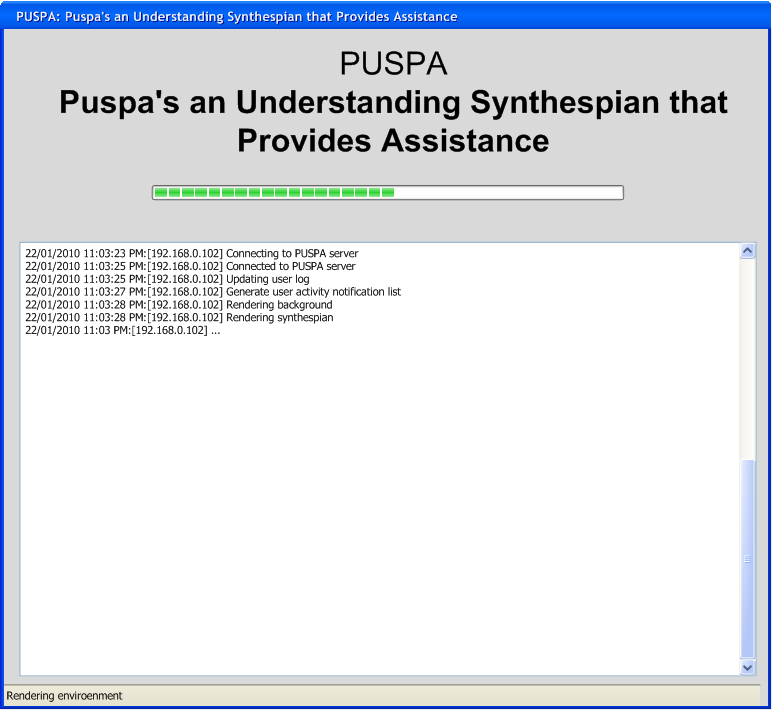
\includegraphics[width=0.6\textwidth]{loading.png}
	\caption{Tampilan antarmuka saat \textit{loading}}
	\label{fig:loading}
\end{figure}
\begin{figure}
	\centering
		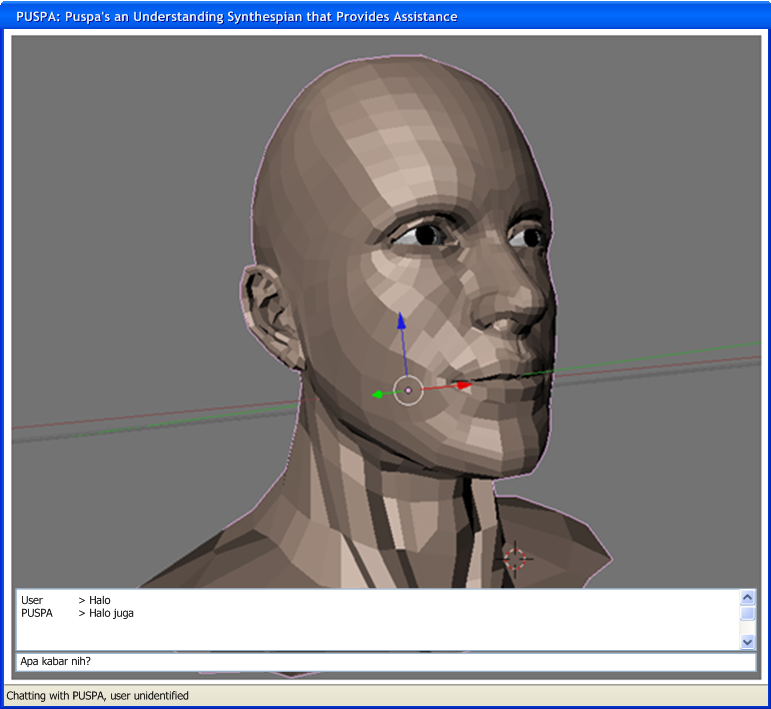
\includegraphics[width=0.6\textwidth]{windowed.png}
	\caption{Tampilan antarmuka dalam jendela (\textit{windowed})}
	\label{fig:windowed}
\end{figure}
\begin{figure}
	\centering
		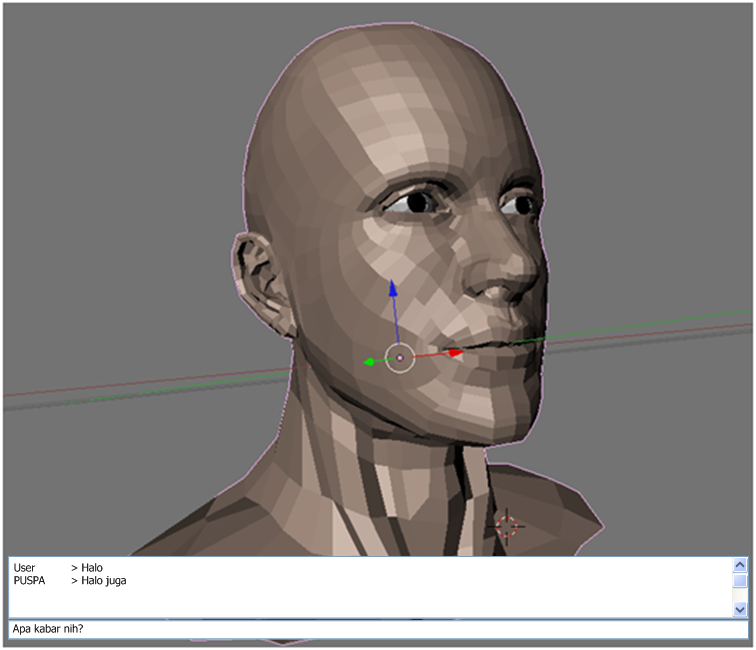
\includegraphics[width=0.8\textwidth]{fullscreen.png}
	\caption{Tampilan antarmuka penuh (\textit{fullscreen})}
	\label{fig:fullscreen}
\end{figure}

\subsection*{\textcolor{subsectioncolor}{\textsf{3. \textit{INTERNAL INTERFACE}}}}
\addcontentsline{toc}{subsection}{3. \textit{INTERNAL INTERFACE}}

\subsubsection*{\textit{System Interface}}
Antarmuka yang dipakai bersama antar subsistem adalah TCP/IP.
Sejauh ini,
subsistem \textit{server} membuka layanannya pada alamat \texttt{rumahtenda.web.id},
dan \textit{port} 12110.
Subsistem \textit{client} hanya harus menyambung ke layanan tersebut,
dan berkomunikasi melalui \textit{port} pilihan sistem operasi \textit{client}.

\subsubsection*{\textit{Subsystem Interface}}
Berikut ini adalah daftar antarmuka tiap modul, beserta penjelasannya.
\begin{itemize}
\item ClientSocket
	\begin{itemize}
	\item\verb!const char* receive();!\\
	yang berfungsi menerima data ketika berkomunikasi dengan \textit{server}.
	\item\verb!void send(const string& output) const;!\\
	yang berfungsi mengirim data ketika berkomunikasi dengan \textit{server}.
	\end{itemize}
\item ServerSocket
	\begin{itemize}
	\item\verb!void listen() const;!\\
	yang berfungsi mendengarkan apakah ada \textit{client} yang menyambung.
	\item\verb!void accept();!\\
	yang berfungsi menerima permintaan sambungan \textit{client}.
	\item\verb!void receive(string& input) const;!\\
	yang berfungsi menerima data ketika berkomunikasi dengan \textit{client}.
	\item\verb!void send(const string& output) const;!\\
	yang berfungsi mengirim data ketika berkomunikasi dengan \textit{client}.
	\end{itemize}
\item NaturalLanguageAnalyser
	\begin{itemize}
	\item\verb!void analyse(const string& input, string& rep);!\\
	yang berfungsi membuat perwakilan makna \texttt{rep} dari masukan \texttt{input}.
	\end{itemize}
\item DialogueManager
	\begin{itemize}
	\item\verb!void respond(const string& input, string& output);!\\
	yang berfungsi membuat tanggapan \texttt{output} dari masukan \texttt{input}.
	\end{itemize}
\item NaturalLanguageGenerator
	\begin{itemize}
	\item\verb!void generate(const string& rep, string& output);!\\
	yang berfungsi membuat keluaran \texttt{output} dari perwakilan makna \texttt{rep}.
	\end{itemize}
\end{itemize}



\section*{\textcolor{sectioncolor}{\textsf{\large DAT: \textit{DATA SPECIFICATION}}}}
\addcontentsline{toc}{section}{DAT: \textit{DATA SPECIFICATION}}

\subsection*{\textcolor{subsectioncolor}{\textsf{1. \textit{INTRODUCTION}}}}
\addcontentsline{toc}{subsection}{1. \textit{INTRODUCTION}}
\hyphenation{di-ki-rim-kan}

\subsubsection*{\texttt{Email}}
Sejauh ini, baru ada satu kelas data, yaitu kelas \texttt{Email}.
Kelas ini memiliki setidaknya empat peubah yaitu alamat pengirim, alamat penerima, judul surat, dan isi surat.

\subsection*{\textcolor{subsectioncolor}{\textsf{2. \textit{DATA TYPES}}}}
\addcontentsline{toc}{subsection}{2. \textit{DATA TYPES}}

\subsubsection*{\texttt{Email}}
Semua peubah \texttt{Email} berjenis \texttt{string}.
Berikut ini gambaran deklarasi peubah-peubah kelasnya.
\begin{verbatim}
class Email
{
private:
  string senderAddr;
  string recipientAddr;
  string subject;
  string content;
};
\end{verbatim}

\subsection*{\textcolor{subsectioncolor}{\textsf{3. \textit{DATA STRUCTURE}}}}
\addcontentsline{toc}{subsection}{3. \textit{DATA STRUCTURE}}

\subsubsection*{\texttt{Email}}

Peubah-peubah dalam \texttt{Email} diberi nilai awal \texttt{string} kosong,
dengan \textit{constructor} berikut.
\begin{verbatim}
Email()
 : senderAddr(""), recipientAddr(""), subject(""), content("")
{
}
\end{verbatim}

Untuk kelas ini, ada \textit{method} \verb!string nextFieldToFill();!,
yang penggunaannya berkaitan dengan PUSPA menanyakan satu-satu nilai bagi tiap peubah yang masih kosong kepada pengguna.
Nilai-nilai itu kemudian dituliskan ke peubah-peubahnya dengan \textit{method} \verb!bool fillNextField(string fillingString);!.



\section*{\textcolor{sectioncolor}{\textsf{\large SSD: \textit{SYSTEM/SUBSYSTEM/MODULE SPECIFICATIONS}}}}
\addcontentsline{toc}{section}{SSD: \textit{SYSTEM/SUBSYSTEM/MODULE SPECIFICATIONS}}

\subsection*{\textcolor{subsectioncolor}{\textsf{1. \textit{INTRODUCTION}}}}
\addcontentsline{toc}{subsection}{1. \textit{INTRODUCTION}}


Secara umum, perangkat lunak PUSPA dapat dibagi menjadi dua subsistem,
yaitu \textit{server} dan \textit{client}.
Secara khusus, perangkat lunak PUSPA dibagi menjadi modul-modul,
dengan fungsi-fungsinya yang ditunjukkan pada Tabel \ref{FungsiPerangkatLunak}.

\begin{table}
	\centering
		\begin{tabular}{|p{1.8cm}|p{4.7cm}|p{8cm}|}
			\hline
				Subsistem & Modul & Keterangan\\
			\hline
				\textit{Server} & NaturalLanguageAnalyser & mengolah bahasa alami\\
				& NaturalLanguageGenerator & membuat kalimat dari tanggapannya\\
				& DialogueManager & membuat tanggapan dan mengatur arah pembicaraan\\
				& TaskManager & melaksanakan tugas\\
				& KnowledgeBase & berperan sebagai pengetahuan PUSPA\\
				& ServerSocket & membuka \textit{port} dan melakukan komunikasi dengan \textit{client}\\
			\hline
				\textit{Client} & Synthespian & model 3D yang berinteraksi dengan pengguna\\
				& UserInterface & menampilkan \textit{user interface} dan interaksinya\\
				& SpeechSynthesiser & melakukan proses TextToSpeech\\
				& FaceDetector & melakukan proses pengenalan wajah dan \textit{tracking}\\
				& SpeechRecogniser & melakukan pengenalan suara (SpeechToText)\\
				& ClientSocket & melakukan komunikasi dengan \textit{server}\\			
			\hline
		\end{tabular}
\caption{Modul-modul dalam PUSPA}
\label{FungsiPerangkatLunak}
\end{table}

\subsection*{\textcolor{subsectioncolor}{\textsf{2. \textit{OVERVIEW}}}}
\addcontentsline{toc}{subsection}{2. \textit{OVERVIEW}}

Menyusul.

\subsection*{\textcolor{subsectioncolor}{\textsf{3. \textit{FUNCTION}}}}
\addcontentsline{toc}{subsection}{3. \textit{FUNCTION}}

Deskripsi fungsi-fungsinya masih sama dengan yang ada pada bagian \textit{Subsystem Breakdown} SFS di B200,
dan yang ditulis pada \textit{header} di \textit{source code} masih sama dengan yang ada pada IFD di dokumen ini.

\subsection*{\textcolor{subsectioncolor}{\textsf{4. \textit{INTERFACES}}}}
\addcontentsline{toc}{subsection}{4. \textit{INTERFACES}}

Masih sama dengan yang ada pada IFD di dokumen ini.

\subsection*{\textcolor{subsectioncolor}{\textsf{5. \textit{STRUCTURES}}}}
\addcontentsline{toc}{subsection}{5. \textit{STRUCTURES}}

\subsubsection*{Deskripsi sistem secara keseluruhan\slash jaringan (\textit{network system configuration})}
\includegraphics[width=0.5\textwidth]{Sistem}

\subsubsection*{Deskripsi subsistem yang ada di dalam sistem (\textit{system block diagram})}
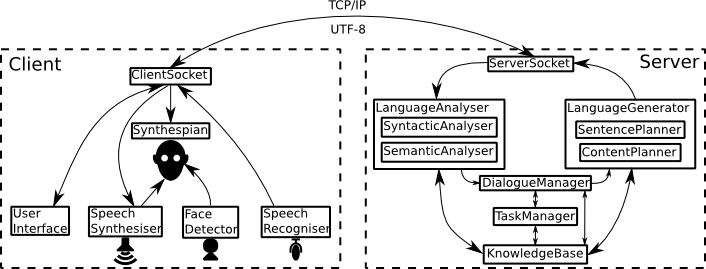
\includegraphics[width=1.0\textwidth]{DiagramBlok}

\subsection*{\textcolor{subsectioncolor}{\textsf{6. \textit{DATA FLOW}}}}
\addcontentsline{toc}{subsection}{6. \textit{DATA FLOW}}

\subsubsection*{Diagram aliran data}
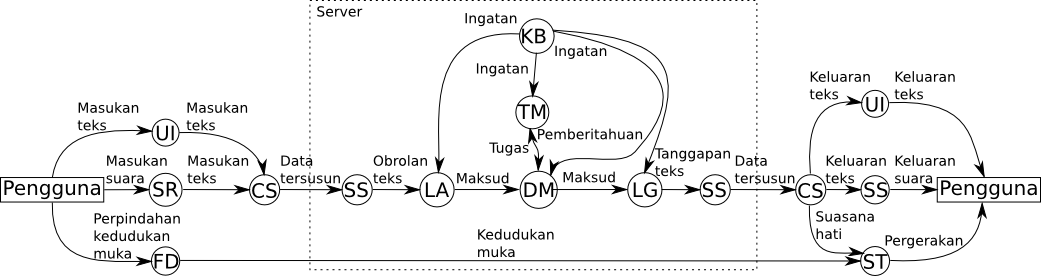
\includegraphics[width=1.0\textwidth]{DiagramAliranData}

\subsection*{\textcolor{subsectioncolor}{\textsf{7. \textit{ENVIRONMENT}}}}
\addcontentsline{toc}{subsection}{7. \textit{ENVIRONMENT}}

Menyusul.



\section*{\textcolor{sectioncolor}{\textsf{\large DEL: \textit{DELTA SPECIFICATION}}}}
\addcontentsline{toc}{section}{DEL: \textit{DELTA SPECIFICATION}}

\subsection*{\textcolor{subsectioncolor}{\textsf{1. \textit{OVERVIEW}}}}
\addcontentsline{toc}{subsection}{1. \textit{OVERVIEW}}

\subsection*{\textcolor{subsectioncolor}{\textsf{2. \textit{DELTA FUNCTIONS DESCRIPTION}}}}
\addcontentsline{toc}{subsection}{2. \textit{DELTA FUNCTIONS DESCRIPTION}}

\subsection*{\textcolor{subsectioncolor}{\textsf{3. \textit{CHANGE OR NEW INTERFACES}}}}
\addcontentsline{toc}{subsection}{3. \textit{CHANGE OR NEW INTERFACES}}

\subsection*{\textcolor{subsectioncolor}{\textsf{4. \textit{MODULE LIST}}}}
\addcontentsline{toc}{subsection}{4. \textit{MODULE LIST}}



\appendix
\addcontentsline{toc}{section}{LAMPIRAN}


\end{document}
